%-------------------------------------------------------------------------------
%	PACKAGES AND OTHER DOCUMENT CONFIGURATIONS
%-------------------------------------------------------------------------------

\documentclass[twoside,twocolumn]{article}

\usepackage{blindtext} % Package to generate dummy text throughout this template

\usepackage[sc]{mathpazo} % Use the Palatino font
\usepackage[T1]{fontenc} % Use 8-bit encoding that has 256 glyphs
\linespread{1.05} % Line spacing - Palatino needs more space between lines
\usepackage{microtype} % Slightly tweak font spacing for aesthetics

\usepackage[english]{babel} % Language hyphenation and typographical rules

%\usepackage[hmarginratio=1:1,top=32mm,columnsep=20pt]{geometry} % Document margins
\usepackage[margin=18mm,top=32mm,columnsep=20pt]{geometry}
\usepackage[hang, small,labelfont=bf,up,textfont=it,up]{caption} % Custom captions under/above floats in tables or figures
\usepackage{booktabs} % Horizontal rules in tables

\usepackage{lettrine} % The lettrine is the first enlarged letter at the beginning of the text

\usepackage{enumitem} % Customized lists
\setlist[itemize]{noitemsep} % Make itemize lists more compact

\usepackage{abstract} % Allows abstract customization
\renewcommand{\abstractnamefont}{\normalfont\bfseries} % Set the "Abstract" text to bold
\renewcommand{\abstracttextfont}{\normalfont\small\itshape} % Set the abstract itself to small italic text

\usepackage{titlesec} % Allows customization of titles
\renewcommand\thesection{\Roman{section}} % Roman numerals for the sections
\renewcommand\thesubsection{\roman{subsection}} % roman numerals for subsections
\titleformat{\section}[block]{\large\scshape\centering}{\thesection.}{1em}{} % Change the look of the section titles
\titleformat{\subsection}[block]{\large}{\thesubsection.}{1em}{} % Change the look of the section titles

\usepackage{fancyhdr} % Headers and footers
\pagestyle{fancy} % All pages have headers and footers
\fancyhead{} % Blank out the default header
\fancyfoot{} % Blank out the default footer
\fancyhead[C]{Deep Learning Seminar $\bullet$ Jan 27, 2021$\bullet$ Deep Reinforcement Learning} % Custom header text
\fancyfoot[RO,LE]{\thepage} % Custom footer text

\usepackage{titling} % Customizing the title section

\usepackage{hyperref} % For hyperlinks in the PDF

\usepackage{graphicx}
\usepackage{amsmath}

\usepackage{csquotes}
\usepackage[
    backend=bibtex,
    style=numeric,
]{biblatex}
\addbibresource{multib.bib}

%-------------------------------------------------------------------------------
%	TITLE SECTION
%-------------------------------------------------------------------------------

\setlength{\droptitle}{-4\baselineskip} % Move the title up

\pretitle{\begin{center}\Huge\bfseries} % Article title formatting
\posttitle{\end{center}} % Article title closing formatting
\title{Deep Reinforcement Learning \\ Actor-Critic and Trust region-based} % Article title
\author{%
\textsc{Andres Becker} \\[1ex] % Your name
\normalsize Technische Universität München \\ % Your institution
\normalsize Fakultät für Mathematik
}
%\date{\today} % Leave empty to omit a date
\date{January 27, 2021}
\renewcommand{\maketitlehookd}{%
\begin{abstract}
\noindent
In recent years, significant progress has been made in solving challenging problems across several fields using Reinforcement Learning (RL). Projects like Deep Mind's AlphaGo Zero \cite{silver2017mastering} have accomplish outstanding results without supervised learning on human knowledge, and showed us the amazing results that RL can achieve. In this small resume, we will focus in a group of RL methods called \emph{Actor-Critic} and the \emph{trust region-based} technique aimed to improve their stability.
\end{abstract}
}

%----------------------------------------------------------------------------------------

\begin{document}

% Print the title
\maketitle

%-------------------------------------------------------------------------------
%	ARTICLE CONTENTS
%-------------------------------------------------------------------------------

\section{What is Reinforcement Learning?}
\lettrine[nindent=0em,lines=3]{W}e refer as Machine learning (ML) to the group of algorithms that improve (learn) automatically through experience. Among this algorithms, we could say that there are three main classes (which depend on the kind of experience we provide):
\begin{itemize}
  \item \textbf{Supervised Learning}: The experience is given in the form of input and output examples, and the goal is to learn a general rule that maps inputs to outputs.
  \item \textbf{Unsupervised Learning}: The experience is given in the form of data (no outputs provided) and the goal is to discover hidden patterns in data.
  \item \textbf{Reinforcement Learning}: No experience (data) is given, instead a dynamic \emph{environment} is provided and an \emph{agent} must learn how to interact with it in order to achieve a goal.
\end{itemize}

\noindent The best way to summarize RL is ``learning by interaction''; An agent interacts with and environment, which in return provides the agent with feedback in form of a reward (see figure \ref{fig:RL_interaction}). Ultimately, the goal of RL is that the agent learns a good (optimal) strategy from experimental trials, and a relative simple received feedback, so that the cumulative rewards is maximized. In reality, the scenario could be a bot playing a game to achieve high scores, or a robot trying to complete physical tasks with physical items.

\begin{figure}
  \centering
  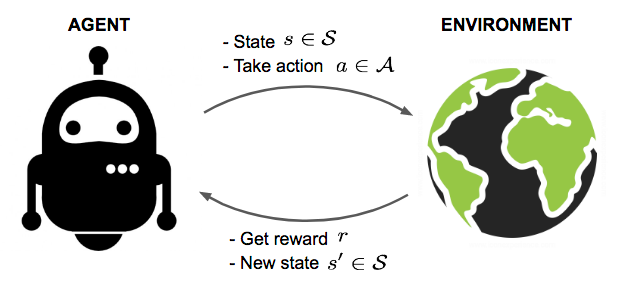
\includegraphics[scale=.24]{Images/RL_illustration.png}
  \caption{Interaction between an Agent and the environment. Image source: \cite{RLsummarylilian}.}
  \label{fig:RL_interaction}
\end{figure}

%------------------------------------------------

\section{Key Concepts of RL}

As we can see in figure \ref{fig:RL_interaction}, the agent interacts with the environment sequentially. Therefore, on time step $t \in \{1,...,T\}$, the agent observe the state of the environment $s_t \in \mathcal{S}$, acts in consequence executing the action $a_t \in \mathcal{A}$, receive its reward $r_t \in \mathcal{R}$ from the environment and observes the new state $s_{t+1} \in \mathcal{S}$.
The tuple $(s_t, a_t, r_t, s_{t+1})$ is known as \emph{transition} step.
This interactions continues until the agent: \textit{i}) Completes the task successfully; \textit{ii}) Fails; \textit{iii}) Reach a time limit. This chain of transition steps from the beginning ($t=1$) until the end ($t=T$) is call \emph{Episode}.
We are interested in environments for which the model that defines them is unknown (\emph{Model-free RL}), and has to be learned explicitly as part of the algorithm (otherwise the optimal solution can be found by means of \emph{Dynamec Programming} (DP)).

\noindent This interaction  is an example of a Markov Decision Process (MDP)\cite{Sutton1998} $\mathcal{M}=(\mathcal{S}, \mathcal{A}, P, R)$, where:

\begin{itemize}
    \item $\mathcal{S}$ is the set of states that holds the Markov property\footnote{The conditional probability distribution of future states (conditional on both past and present states) depends only upon the present state, not on the sequence of events that preceded it, i.e. $P(s_{t+1}|s_{t}, s_{t-1},\dots, s_1)=P(s_{t+1}|s_{t})$.}.
    \item $\mathcal{A}$ is the set of actions.
    \item $P$ is the transition probability function: $P(s_{t+1},r_{t+1}|s_t, a_t)$.
    \item $R$ is the reward function: $R(s_t, a_t):=\mathbb{E}[R_{t+1}|s_t,a_t]=\sum_{r\in \mathcal{R}}r \sum_{s' \in \mathcal{S}}P(s',r|s_t, a_t)$.
\end{itemize}

However, note that in fact we are not interested in maximizing the reward on each time step but the \emph{Return} instead, which is the future cumulative reward\footnote{This might sound counterintuitive. However, think of it as when you have to make less rewarding decisions in the short term (e.g. watching Netflix instead of studying) in order to achieve a greater long-term goal (e.g. approving an exam).}:
\begin{equation}
  G_t := \sum_{k=0}^T \gamma^k r_{t+k+1}
\end{equation}
where $\gamma \in [0,1]$ is the discount factor meant to encourage the agent to finish the task as soon as possible, since in practice time is a valuable resource.

Recall that the ultimate goal of RL is to find an optimal strategy, such that it maximize the Return. Then, how to choose actions that help us to achieve this? The answer is the \emph{Policy} $\pi$. The policy is the functions that defines the agent’s behavior and maps a state $s$ to an action $a$. This function can be either deterministic or stochastic:

\begin{itemize}
  \item \textbf{Deterministic}: $\pi: \mathcal{S} \rightarrow \mathcal{A}$; i.e. $\pi(s)=a$.
  \item \textbf{Stochastic}: $\pi: \mathcal{S} \times \mathcal{A} \rightarrow [0, 1]$; i.e. $\pi(a|s)=P_{\pi}(A=a|S=s)$.
\end{itemize}

Now that we have (more or less) a clear idea of what RL seeks (maximize the return $G$) and how to do it (by finding an optimal policy $\pi$), we need to define a way to quantify how good a state $a$ is (in terms of the return $G$) in a given environment (when we follow a policy $\pi$), and how good an action $a$ is (in terms of the return $G$) when the environment is in state $s$ (and when we follow a policy $\pi$). This is done through the \emph{State-value} and \emph{Action-value} functions respectively:
\begin{itemize}
    \item \textbf{State-value}: $V_{\pi}(s):= \mathbb{E}_{\pi}[G_t|s_t=s]$.
    \item \textbf{Action-value}: $Q_{\pi}(s, a):= \mathbb{E}_{\pi}[G_t|s_t=s, a_t=a]$.
\end{itemize}


mover esto a action value section, ya que la v ahora va a tener parametros w


\begin{equation}
  A_{\pi}(s,a):=Q_{\pi}(s, a) - V_{\pi}(s)
\end{equation}

\noindent However, the Action-value function tell us how valuable and action is w.r.t. the long term (return). But, what if we only want to know the value that taking the action $a$ (following the policy $\pi$) could bring in the short term (i.e. when it is executed in an environment to go from state $s$ to the next one $s'$)? This question is answered by the \textbf{Advantage} function:

\begin{equation}
  A_{\pi}(s,a):=Q_{\pi}(s, a) - V_{\pi}(s)
\end{equation}


%-------------------------------------------------------------------------------

\section{Policy Gradient methods}

There are several ways to approximate an optimal strategy. For example, in \emph{action-value} methods we learn the values of actions and then select
actions based on their estimated action values (e.g. \textit{Q-learning}). Nevertheless, this means that their policies would not even exist without the action-value estimates \cite{Sutton1998}.

However, in \emph{Policy Gradient} we consider methods that instead learn a parameterized policy (e.g. an artificial neural network) that can select actions without consulting a value function\footnote{A value function may still be used to learn the policy parameter, but is not required for action selection.}.
Therefore, we write
$$\pi(a|s,\boldsymbol{\theta}) = Pr(A_t=a | S_t=s; \boldsymbol{\theta}_t=\boldsymbol{\theta})$$
 to denote the probability that the action $a$ is taken, given the parameters $\boldsymbol{\theta}$ and that the environment is in state $s$ at time $t$.
Then, we can approximate an optimal policy by means of gradient ascent while maximizing a performance measure $J(\boldsymbol{\theta})$:

\begin{equation}
  \boldsymbol{\theta}_{t+1} = \boldsymbol{\theta}_{t} + \widehat{\alpha \nabla J(\boldsymbol{\theta}_t)}
  \label{eq:learn_rule}
\end{equation}

\noindent where $\widehat{\nabla J(\boldsymbol{\theta})}$ is a stochastic unbiased estimator of $\nabla J(\boldsymbol{\theta})$ (i.e. $\mathbb{E}[\widehat{\nabla J(\boldsymbol{\theta})}] = \nabla J(\boldsymbol{\theta})$).

Then, how to define the performance measure $J(\boldsymbol{\theta})$?
There are many ways to define $J$, which depend mainly on the method used to approximate the policy.
However, since we are considering only episodic environments\footnote{The definition and explanation of the continuous case is out of the scope of this work.}, then we seek to maximize the return in a given time step ($G_t$), and therefore we define it as the value of the state $s_t$ , i.e. $J(\boldsymbol{\theta}):=V_{\pi_{\boldsymbol{\theta}}}(s_t)$.

Since we are approximating an optimal policy, we need to express $\nabla J(\boldsymbol{\theta})$ in terms of $\pi(\boldsymbol{\theta})$. Therefore, after marginalize $V_{\pi_{\boldsymbol{\theta}}}(s_t)$ over the action space $\mathcal{A}$ and applying Baye's rule we have:

\begin{equation}
  \begin{split}
    \nabla J({\boldsymbol{\theta}}) &= \nabla V_{\pi_{\boldsymbol{\theta}}}(s_t)\\
    &= \nabla \sum_{a_t \in \mathcal{A}} \pi (a_t|s_t; \boldsymbol{\theta}) Q_{\pi_{\boldsymbol{\theta}}}(s_t,a_t)
  \end{split}
  \label{eq:grad}
\end{equation}

The problem is that the right hand side of equation \ref{eq:grad} depends on both the action selections and the distribution of states in which those selections are made, and that both of these are affected by the policy parameter. Fortunately, with the aid of the \emph{Policy Gradient Theorem} we can reformulate $\nabla J({\boldsymbol{\theta}})$ to be proportional to $\nabla \pi (a_t|s_t; \boldsymbol{\theta})$\footnote{A complete proof to this result can be found in page 325 of \cite{Sutton1998}.}:

\begin{equation*}
\resizebox{.95\linewidth}{!}{%
  $\begin{split}
    \nabla J({\boldsymbol{\theta}}) &\propto
    \sum_{s_t \in \mathcal{S}} \mu (s_t) \sum_{a_t \in \mathcal{A}} Q_{\pi_{\boldsymbol{\theta}}}(s_t,a_t) \nabla \pi (a_t|s_t; \boldsymbol{\theta}) \\
    &=\sum_{s_t \in \mathcal{S}} \mu (s_t) \sum_{a_t \in \mathcal{A}} \pi (a_t|s_t; \boldsymbol{\theta}) Q_{\pi_{\boldsymbol{\theta}}}(s_t,a_t) \frac{\nabla \pi (a_t|s_t; \boldsymbol{\theta})}{\pi (a_t|s_t; \boldsymbol{\theta})} \\
    &=\sum_{s_t \in \mathcal{S}} \mu (s_t) \sum_{a_t \in \mathcal{A}} \pi (a_t|s_t; \boldsymbol{\theta}) Q_{\pi_{\boldsymbol{\theta}}}(s_t,a_t) \nabla \log{\pi (a_t|s_t; \boldsymbol{\theta})} \\
    &= \mathbb{E}[Q_{\pi_{\boldsymbol{\theta}}}(S_t,A_t) \nabla \log{\pi (A_t|S_t; \boldsymbol{\theta})}] \\
    &= \mathbb{E}[G_t \nabla \log{\pi (A_t|S_t; \boldsymbol{\theta})}] \\
  \end{split}
  $}
\end{equation*}


\noindent where $\mathbb{E}$ is the expectation over the distribution of states $\mu(s_t)$ and actions $\pi (a_t|s_t; \boldsymbol{\theta})$; $A_t$ and $S_t$ are random variables ($A_t \sim \mu(s_t)$ and $S_t \sim \pi (a_t|s_t; \boldsymbol{\theta})$); and $Q_{\pi_{\boldsymbol{\theta}}}(S_t,A_t)$ can be replaced by $G_t$ since $\mathbb{E}[G_t| S_t,A_t] = Q_{\pi_{\boldsymbol{\theta}}}(S_t,A_t)$.

Therefore, our learning rule defined in \ref{eq:learn_rule} can be updated to:

\begin{equation*}
  \boldsymbol{\theta}_{t+1} = \boldsymbol{\theta}_{t} + \alpha G_t \nabla \log{\pi (A_t|S_t; \boldsymbol{\theta})}
\end{equation*}

However, the \emph{Policy Gradient Theorem} can be generalized to include a comparison of the action value to an arbitrary baseline $b(s)$ \cite{Sutton1998}, which can be any function, even a random variable, as long as it does not vary with a:

\begin{equation*}
  \nabla J({\boldsymbol{\theta}}) \propto
  \sum_{s_t \in \mathcal{S}} \mu (s_t) \sum_{a_t \in \mathcal{A}} \left( Q_{\pi_{\boldsymbol{\theta}}}(s_t,a_t) - b(s_t) \right) \nabla \pi (a_t|s_t; \boldsymbol{\theta})
\end{equation*}

the last equation remains valid because the subtracted quantity is zero:

\begin{equation*}
  \begin{split}
    \sum_{a_t \in \mathcal{A}} b(s_t) \nabla \pi (a_t|s_t; \boldsymbol{\theta}) &=
    b(s_t) \sum_{a_t \in \mathcal{A}} \nabla \pi (a_t|s_t; \boldsymbol{\theta})\\
    &= b(s_t) \nabla 1 \\
    &= 0
  \end{split}
\end{equation*}

Finally, we can use this to derive a new update rule that includes a general baseline:

\begin{equation}
  \boldsymbol{\theta}_{t+1} = \boldsymbol{\theta}_{t} + \alpha (G_t - b(S_t)) \nabla \log{\pi (A_t|S_t; \boldsymbol{\theta})}
  \label{eq:learn_rule_bl}
\end{equation}

%-------------------------------------------------------------------------------

\section{Actor-Critic}

poner aqui la foto del video (el diagrama de ben)

Moreover, we can also learn the value function as well.

Therefore, the \emph{Actor} refers to the policy and the \emph{Critic} to the estimate of the value function. In deep RL, both the actor and the critic can be represented by non-linear neural networks function approximators \cite{mnih2016asynchronous}.
 In the same way, $\boldsymbol{W}$ denote the parameters of the function used to learn the value function.

We denote the \emph{Expected Cumulative Reward} as $J(\boldsymbol{\theta})$, since we seek to maximize it depending on the parameters of the policy $\pi_{\boldsymbol{\theta}}$. Therefore, we can use \emph{Gradient ascent} in $J$ to maximize the performance of the policy:
\begin{equation}
  \boldsymbol{\theta}_{t+1} = \boldsymbol{\theta}_{t} + \alpha \nabla J(\boldsymbol{\theta}_t)
\end{equation}

define quien es el actor, el critic y la advantage (tal vez tendras que pasar la explicacion que ya diste de la q function a la v)

ahora especifica la regla del gradient acent para el actor

para el critic no es necesario (o es directo) puesto que es un problema de regrecion por lo que mse.

por ultimo escribe el algoritmo para actor-critic

\section{Trust region-based}

algo no muy largo

%-------------------------------------------------------------------------------
%	REFERENCE LIST
%-------------------------------------------------------------------------------

\printbibliography

%-------------------------------------------------------------------------------

\end{document}
